\subsection{Graphical User Interface}
\label{subsec:gui}

The graphical user interface, or GUI for short, was meant to be simple and intuitive to use. In the end, that requirement turned into the navigation chart seen in \ref{fig:application_navigation}. The interface is mostly split into four different areas. One is the login, consisting of a login and sign-up screen. The other is the "Main Menu" of the application. This screen can be swiped to the side to show any of the five sub-screens associated with it. The third is instances of recipes, displaying both the recipe and any comments made to it. Last is the recommendation part meant to visualize suggestions, helping the user to choose the best one.

The following will give a more detailed description as to the purpose of the GUI components.

\begin{figure}[H]
	\centering
	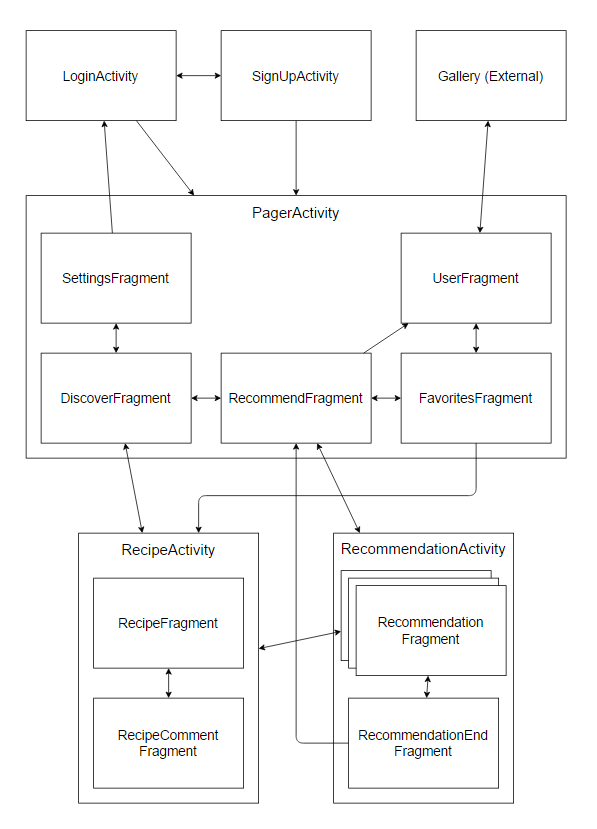
\includegraphics[width=\textwidth]{Pictures/application_navigation.png}
	\caption{Navigation paths in the application}
	\label{fig:application_navigation}
\end{figure}

\paragraph{Login- And SignUpActivity}
When launching the application, the \texttt{LoginActivity} is the point of entry. This obviously serves the purpose of logging the user into the application, but also enables the storage and retrieval of certain information under that particular user. Information about this can be seen in \todo{noget der ikke er skrevet endnu}. Furthermore, if the user has already logged in once, the \texttt{LoginActivity} is skipped entirely, launching the \texttt{PagerActivity} instead. This eases the use of the application, since users only have to login once. They will then stay logged in unless they manually log out.

For users who have not signed up yet, the \texttt{LoginActivity} features a link to the \texttt{SignUpActivity}. Through here, the user can create a new account. Besides from this, the functionality is similar to \texttt{LoginActivity}. Both screens feature a "Sign Up"/"Login" button, taking the user to the main user interface, the \texttt{PagerActivity}.

\paragraph{PagerActivity}
This \texttt{Activity} can be seen as the "Main Menu" of the application and features two elements. The first is the \texttt{ViewPager}. This is an Android component that allows \texttt{View} instances to be "paged". This allows the user to slide the views left or right, with another view coming into the screen. This can be read about at \todo{cite something}.

This particular \texttt{ViewPager} holds five different \texttt{Fragment} instances. A \texttt{Fragment} is similar to an \texttt{Activity}. It has its own layout and lifecycle, but is possible to manipulate within a running \texttt{Activity}.\todo{cite something} For the purpose of this project, the fragments could have been an entire \texttt{Activity} each. But given the goal of making the GUI as fluent and simple as possible, using a \texttt{ViewPager} was a good way of eliminating excessive amounts of buttons and loading between five different \texttt{Activity} instances. \texttt{VievPager} does however use additional memory since it pre-loads the nearest fragments. For example, if \texttt{Fragment} 3 is currently shown to the user, \texttt{Fragment} 2 and 4 are also in memory, ready to slide onto the screen. This was however considered an acceptable trade-off.

The second element of the \texttt{PagerActivity} is a simple navigation bar, showing which window is currently shown, and letting the user press an icon to change the window. This exists for two reasons. One is to create a shortcut for the user. As worst example, going from the first \texttt{Fragment} to the last would require four swipes, which is now doable with one press. It is also to ensure that the user understands the navigation. Sliding on the screen is easy, but since only one \texttt{Fragment} is visible at a time, users can not know about the feature otherwise.

\paragraph{RecommendFragment}

\paragraph{UserFragment}

\paragraph{FavoriteFragment}

\paragraph{DiscoverFragment}

\paragraph{SettingsFragment}

\paragraph{RecommendationActivity}

\paragraph{RecipeActivity}